\chapter{Practical Application}

This chapter presents the practical application of functional package management and
containerization technologies through the development and deployment of a stateless
web server written in the Rust programming language \cite{RustProgrammingLanguage}.
The primary objective is to demonstrate the effectiveness, challenges, and benefits
of using functional package management and containerization technologies in a real-world
project. While Nix and Docker are the specific tools selected for this implementation,
the emphasis is on the general principles and methodologies of functional package
management and containerization technologies, rather than the tools themselves.

The web server in question serves both static and dynamic content. Although the server’s
functionality is relatively straightforward, it is well-suited for illustrating modern
practices in environment management and deployment workflows. The server fetches data
from an API and returns web content in HTML, utilizing HTMX for dynamic interaction
\cite{HtmxHighPower} and Tailwind CSS for styling \cite{TailwindCSSRapidly2020}. This
project aims to highlight the integration of functional package management and
containerization technologies, focusing on how they manage dependencies, ensure
reproducible builds, and facilitate the deployment of the application in an isolated
environment. The complete source code is publicly available on GitHub
\cite{hornClemenscodesWebserver2024}, allowing for replication of the setup.

The practical importance of this project lies not in the complexity of the web server
itself, but in the techniques used to manage the server’s development and deployment
environments. One of the primary challenges addressed in this project is the management
of specific compile-time dependencies, such as OpenSSL, which are required for building
the server. These dependencies provide an ideal scenario for demonstrating how functional
package management handles complex build environments while ensuring reproducibility.
Additionally, this project enables a comparison of how functional package management
and containerization technologies contribute to modern development workflows, with a
focus on key aspects such as ease of use, build times, environment isolation, and
reproducibility.

This chapter is structured progressively, beginning with detailed instructions on
setting up the development environments using both functional package management and
containerization technologies. This includes installing and configuring Nix for functional
package management and Docker for containerization, with specific attention to how these
tools are used on various platforms, such as Linux or Windows.
Following the installation process, the chapter covers how to integrate these technologies
into IDEs like Visual Studio Code,
which improves productivity by allowing the developer to manage dependencies, run builds,
and isolate environments directly from the IDE.
Next, the chapter demonstrates how each technology was utilized to build and run the web
server using best practices. Nix was employed for managing dependencies and ensuring
reproducibility in development environments, while Docker was used to package the
application into containers for deployment. Code snippets are provided to show how the
technologies were configured, and best practices are highlighted to ensure that the
development and deployment processes are efficient and reliable.
The chapter concludes with a section on CI/CD pipelines,
configured using GitHub Actions. Separate workflows were created for
functional package management and containerization technologies, allowing for a comparison
of their performance in automated testing and deployment environments. Each workflow is
explained in detail, showing how both approaches can be integrated into modern CI/CD pipelines.

This chapter serves as the foundation for the analysis presented in the next chapter, which
will delve deeper into the comparative evaluation of functional package management and
containerization technologies. Here, the focus remains on the practical steps taken, while
the analysis of their respective strengths, weaknesses, and impacts on development workflows
will follow.

\section{Setup}

Setting up a reproducible development environment is crucial for ensuring consistency
and reliability in software development, especially when working across various
platforms and with diverse team members. In this section, we focus on two
specific tools: Nix and Docker, which serve as examples of functional package
management and containerization technologies, respectively. Both tools play a
vital role in modern development workflows, ensuring that development
environments can be recreated accurately, no matter where they are deployed.

The following command installs Nix as a multi-user system
on Unix-based systems such as Linux and macOS.

\begin{lstlisting}[caption={Installing Nix on Linux and macOS}]
sh <(curl -L https://nixos.org/nix/install) --daemon
\end{lstlisting}

After installation, Nix must be integrated into the user's shell environment to
make its commands available. This is done by sourcing the Nix configuration file,
which is automatically generated during installation. This step ensures that the `nix`
command and its associated functionalities are accessible within the current shell session.

\begin{lstlisting}[caption={Configuring Shell for Nix}]
source /nix/var/nix/profiles/default/etc/profile.d/nix-daemon.sh
\end{lstlisting}

For Windows users, Nix is not natively supported but can be run using the Windows
Subsystem for Linux (WSL). WSL provides a Unix-like environment on Windows systems,
allowing users to install and run Linux applications natively. The same installation
procedure used on Linux applies within the WSL environment, making it possible for
Windows users to leverage the functional package management capabilities of Nix.

Once installed and configured, Nix allows users to define their entire development
environment in a single configuration file (e.g., `default.nix`). This file specifies
the exact versions of all required dependencies, ensuring that the environment can
be reproduced across different machines. The ability to roll back environments to
previous states also helps mitigate issues that might arise during software updates.

To install Docker on Linux,
users can utilize their system’s package manager. For Debian-based systems,
the following commands will install Docker and set up permissions so that users can
run Docker without needing superuser privileges:

\begin{lstlisting}[caption={Installing Docker on Linux}]
sudo apt-get update
sudo apt-get install docker-ce docker-ce-cli containerd.io
sudo usermod -aG docker $USER
newgrp docker
\end{lstlisting}

For Windows users, Docker Desktop is available, which uses WSL2 as the backend to
run containers. After installing Docker Desktop, users can interact with Docker
via its GUI or command-line tools. Docker Desktop also
handles system-level configurations for networking and storage, making it easier
to manage containers on Windows systems.

In summary, the setup of development environments using Nix and Docker ensures
that both package-level and runtime dependencies can be managed in a reproducible
and isolated manner. These tools form the foundation of reproducible development
workflows, ensuring that development environments can be easily recreated across
different systems and stages of software development.

\section{Development Environment Configuration}

In software development, creating a reproducible and isolated development
environment is essential for ensuring consistency across different systems
and developers. This section discusses how to utilize two key technologies for
setting up such environments: functional package management and containerization.
The goal is to create development environments that are isolated from the host
system, ensuring consistency in the development process regardless of the
developer's operating system or machine configuration.

The following subsections will discuss each approach in detail, starting with
functional package management and its role in setting up development environments.

\subsection{Functional Package Management for Development Environments}

In a functional package management system, such as Nix, developers can define their
entire development environment, including compilers, libraries, tools, and other
dependencies, in a single configuration file. This file describes the precise
version of every component needed for development and testing.

Below is an example of how this can be achieved using a configuration file. While
the following implementation is specific to Nix, the concepts are general and can
be applied to other functional package management systems. The file defines inputs,
which include external resources like package repositories and overlays for specific
languages or tools.

\begin{lstlisting}[caption={Input section for functional package management}]
{
  inputs = {
    nixpkgs.url = "github:NixOS/nixpkgs/nixos-unstable";
    flake-utils.url = "github:numtide/flake-utils";
    nix-filter.url = "github:numtide/nix-filter";
    rust-overlay = {
      url = "github:oxalica/rust-overlay";
      inputs.nixpkgs.follows = "nixpkgs";
    };
  };
\end{lstlisting}

In this example, the inputs define the external sources required to build the
environment. The main idea is that the package repository (here represented by
nixpkgs) and overlays (such as rust-overlay) provide packages in a purely
functional manner, ensuring that different versions of packages can coexist without
conflicts. The configuration guarantees that the exact same packages will be
used by all developers working on the project.

The outputs section defines what is produced by the functional package management
system, including development shells. A development shell is an isolated environment
that includes all the tools and dependencies needed for development. By defining
such environments declaratively, functional package managers ensure that all
developers have access to the same setup.

\begin{lstlisting}[caption={Outputs section for functional package management}]
  outputs = inputs:
    with inputs;
      flake-utils.lib.eachDefaultSystem (
        system: let
          inherit (nixpkgs) lib;
          overlays = [(import rust-overlay)];
          filter = nix-filter.lib;
          pkgs = import nixpkgs { inherit system lib overlays; };
          bin = pkgs.pkgsBuildHost.rust-bin;
          rustToolchain = bin.fromRustupToolchainFile ./rust-toolchain.toml;
\end{lstlisting}

The outputs are built in a way that respects the functional programming paradigm.
This means that each output is a pure function of its inputs, and any change in the
input will result in a predictable change in the output. For example, a change in
the rust-overlay version will result in a new environment that reflects that
specific version of Rust, without affecting other environments that rely on a
different version.

Functional package management systems also allow the definition of development
shells, which are isolated environments that provide all the tools and dependencies
needed for development. These shells are constructed based on the inputs and outputs
defined in the configuration file.

\begin{lstlisting}[caption={Development shell for functional package management}]
            devShells = {
              default = mkShell {
                buildInputs = [pkg-config];
                nativeBuildInputs = [
                  extendedRustToolchain
                  rust-analyzer
                  openssl
                  proto
                  moon
                ];
                RUST_SRC_PATH =
                "${rust.packages.stable.rustPlatform.rustLibSrc}";
                RUST_BACKTRACE = 1;
                shellHook = ''echo "Entering the development shell..."'';
              };
            };
\end{lstlisting}

The development shell isolates the environment, ensuring that any tools or
libraries installed in the shell do not interfere with the global system.
Furthermore, each shell is defined declaratively, meaning that it can be shared
among developers, ensuring that everyone works in the same environment.

In addition to specifying the dependencies, functional package management allows
the definition of environment variables. These variables can be defined inside the
development shell configuration and will be automatically set whenever the shell is
entered. In the example above, the \texttt{RUST\_SRC\_PATH} variable is set to
point to the Rust standard library source, and the \texttt{RUST\_BACKTRACE} variable
is enabled to assist with debugging by providing detailed backtrace information.

Another powerful feature provided by functional package management systems like
Nix is the ability to define \textit{shell hooks}. A shell hook is a script that
runs as soon as the development shell is entered. This can be used to run
initialization scripts, set up additional configuration, or prepare the environment
for specific tasks.

In this example, a shell hook is defined, which prints a message and sets a custom
environment variable.
Shell hooks can be a powerful tool for automating setup tasks and ensuring
the environment is properly initialized for development.

Functional package management systems also support binary caching, allowing
developers to reuse pre-built binaries across different environments and machines.
This significantly speeds up the process of setting up a development environment,
as pre-built binaries can be fetched from a cache instead of being built locally.

\begin{lstlisting}[caption={Cachix configuration for functional package management}]
  nixConfig = {
    extra-substituters = [
      "https://nix-community.cachix.org"
      "https://clemenscodes.cachix.org"
    ];
    extra-trusted-public-keys = [
      "nix-community.cachix.org-1:mB9FSh9qf2dCimDSUo8Zy7bkq5CX+/rkCWyvRCYg3Fs="
      "clemenscodes.cachix.org-1:yEwW1YgttL2xdsyfFDz/vv8zZRhRGMeDQsKKmtV1N18="
    ];
  };
\end{lstlisting}

By incorporating binary caching into the functional package management process,
developers can avoid the time-consuming task of building every package from source,
while still ensuring that the environment remains reproducible and isolated.

In summary, functional package management provides a powerful and flexible way to
define development environments. By isolating dependencies and ensuring that
environments are fully reproducible, developers can avoid conflicts and inconsistencies
across different machines, ensuring that the development process remains smooth and
predictable.

In the next subsection, we will discuss how containerization, particularly with
Docker Devcontainers, can be used to achieve similar isolation and reproducibility.

\subsection{Containerization for Development Environments}

Containerization is an important concept in modern software development, enabling
the creation of isolated, reproducible environments. The idea behind containerization
is to package not only the application code but also its dependencies, runtime, and
system libraries into a single image. This ensures that the environment will behave
consistently, regardless of where it is deployed. Docker is one of the most widely
used technologies for implementing containerization. Docker containers encapsulate
everything needed to run an application, isolating it from the host system and other
running applications.

In the context of development environments, containerization is particularly useful
because it guarantees that developers work with the same tools, configurations, and
dependencies, eliminating issues that may arise from differences between local setups.
The concept of immutability is central to containerization: containers are built from
immutable images, ensuring that the environment does not change unexpectedly once it
is created.

The Visual Studio Code Dev Containers extension allows developers to use a container
as a fully-featured development environment. By isolating the development environment
inside a container, it ensures that the tools, libraries, and configurations remain
consistent across different systems. This is particularly useful in collaborative
projects or when working with complex dependencies. A \texttt{devcontainer.json}
file is used to define how Visual Studio Code accesses or creates a development
container with the necessary toolchain and runtime stack. The container can be used
to run the application, compile libraries, or provide separate runtimes needed
for interacting with the codebase.

Workspace files are either mounted from the local file system into the container
or cloned directly into it. This ensures that developers can seamlessly interact
with the containerized environment while retaining access to the entire workspace
from the host system. Extensions are installed and executed inside the container,
providing full access to the tools, platform, and file system inside the container.

As a result, developers can switch between development environments by simply
connecting to a different container, without having to worry about reconfiguring
tools or dependencies locally.

The diagram below illustrates the interaction between the local operating system,
Visual Studio Code, and the containerized environment:

\begin{figure}[H]
	\centering
	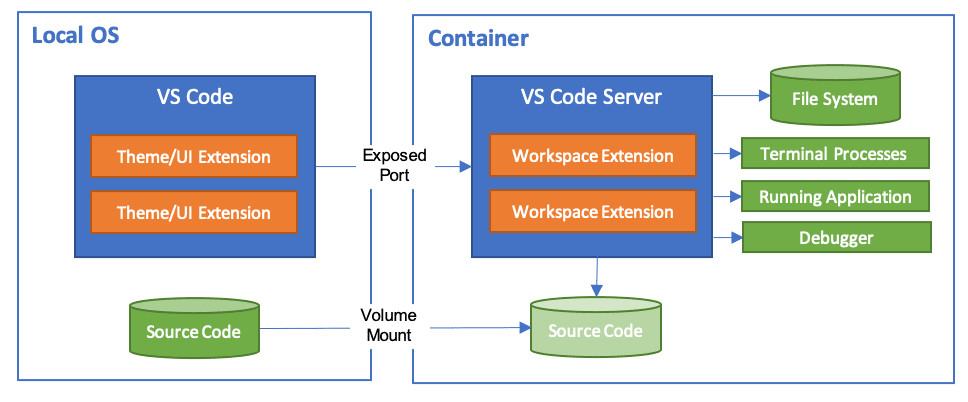
\includegraphics[width=0.9\textwidth]{assets/images/architecture-containers.png}
	\caption{Devcontainer Architecture: VS Code and Docker Integration \cite{DevelopingContainerUsing}}
\end{figure}

In this architecture, Visual Studio Code, running on the local machine, provides the
interface for the developer to interact with the container. The local machine runs
UI-related extensions such as themes, while the container hosts the VS Code server
and manages all the runtime tasks.
Inside the container, developers have access to
the file system, terminal processes, application runtimes, and debugging capabilities.
The workspace files, including the source code, are mounted from the local system
into the container using a volume mount, allowing seamless interaction with the code
from within the container. Exposed ports allow services running inside the container,
such as web servers, to be accessed from the local machine.

This setup ensures a local-quality development experience while providing all the
benefits of containerized isolation. Developers can perform tasks such as
code navigation, IntelliSense, and debugging without worrying about conflicts with
local environments. Visual Studio Code can run in two primary modes with Dev Containers:
as a full-time development environment inside the container, or by attaching to a
pre-existing running container for inspection or debugging purposes.

By leveraging Dev Containers, developers can ensure a consistent, isolated development
workflow while benefiting from the reproducibility and portability that Docker containers
offer. This integration streamlines the process of setting up a development environment,
making it easier to manage complex dependencies and configurations in a unified,
containerized workspace.

\subsubsection{Devcontainer Setup for Development Environments}

The Devcontainer setup used for this application highlights the power of
containerization technologies in creating a consistent and isolated development
environment. The setup consists of three key files: \texttt{devcontainer.json},
\texttt{Dockerfile}, and \texttt{.vscode/extensions.json}. Together, these files
configure the containerized development environment, providing developers with all
the necessary tools and dependencies without affecting the host system. By using a
container, the development environment remains reproducible across different machines,
ensuring consistency throughout the project lifecycle. Although this example uses
Visual Studio Code Dev Containers, the underlying principles of containerization—such
as environment isolation and dependency management—remain relevant across different
tools and technologies.

The \texttt{devcontainer.json} file is the cornerstone of this setup. It defines
how the development container is built and managed, specifying important parameters
such as the Dockerfile location, port forwarding, and workspace mounting. The following
is the configuration used for the Rust project:

\begin{lstlisting}[caption={devcontainer.json Configuration}]
{
  "name": "Rust Development Container",
  "build": {
    "dockerfile": "Dockerfile",
    "context": ".."
  },
  "forwardPorts": [
    8000
  ],
  "mounts": [
    "source=${localWorkspaceFolder},target=/app,type=bind"
  ]
}
\end{lstlisting}


This file defines several key aspects of the containerized environment. The
\texttt{dockerfile} attribute specifies the Dockerfile used to build the container,
while the \texttt{context} is set to the parent directory. This allows Docker to
access all the files needed to construct the environment. The \texttt{forwardPorts}
section ensures that port 8000 from within the container is accessible on the host
system, facilitating local testing of web applications. Finally, the \texttt{mounts}
section binds the local workspace folder to the \texttt{/app} directory within the
container, ensuring that changes made on the host machine are immediately reflected
inside the container. In this setup, the local workspace directory, represented
by the \texttt{\${localWorkspaceFolder}} variable, is bound to the \texttt{/app}
directory inside the container

The \texttt{Dockerfile} is used to create the containerized environment. In this
case, the Dockerfile is designed specifically for development purposes, optimizing
for flexibility and ease of use rather than production deployment. It defines the
base environment, installs necessary tools, and configures additional settings that
are critical for Rust development. Below is the Dockerfile used in this project:

\begin{lstlisting}[caption={Development Dockerfile for Rust Project}]
FROM rust:1.80.1-slim-bullseye

ENV DEBIAN_FRONTEND=noninteractive
ENV SHELL=/bin/bash
ENV PATH="/root/.proto/bin:$PATH"

RUN apt-get update && \
  apt-get install -y --no-install-recommends \
  git=1:2.30.2-1* \
  gzip=1.10-4* \
  unzip=6.0-26* \
  xz-utils=5.2.5-2.1* \
  curl=7.74.0-1.3* \
  pkg-config=0.29.2-1* \
  openssl=1.1.1* \
  libssl-dev=1.1.1* \
  musl-tools=1.2.2-1* \
  make=4.3-4.1* \
  && \
  apt-get clean && \
  rm -rf /var/lib/apt/lists/*

SHELL ["/bin/bash", "-o", "pipefail", "-c"]

RUN curl -fsSL https://moonrepo.dev/install/proto.sh | \
    bash -s -- 0.40.4 --yes && \
    proto plugin add moon \
    "https://raw.githubusercontent.com/moonrepo/moon/master/proto-plugin.toml" && \
    proto install moon

WORKDIR /app

COPY .moon .moon
COPY .prototools .prototools
COPY dockerManifest.json dockerManifest.json
COPY moon.yml moon.yml

RUN moon docker setup && \
    cargo install cargo-watch --locked
\end{lstlisting}

The Dockerfile begins by using the official Rust image \texttt{rust:1.80.1-slim-bullseye},
which ensures that the Rust toolchain is available within the container. Key environment
variables are defined to streamline the package installation process and configure the
shell. A series of packages are installed using \texttt{apt-get}, including Git, OpenSSL,
and \texttt{pkg-config}, which are necessary for building and testing Rust applications.

Next, the \texttt{moonrepo} tool is installed via the Proto installer, a tool used to
manage project workflows and tasks. This enables the environment to manage project tasks
efficiently. The Dockerfile also sets the working directory to \texttt{/app}, where the
local workspace is mounted. Various configuration files, such as \texttt{moon.yml} and
\texttt{dockerManifest.json}, are copied into the container. Lastly, the \texttt{moon}
tool is configured, and \texttt{cargo-watch} is installed to monitor file changes,
providing a productive development experience with real-time feedback.

The \texttt{.vscode/extensions.json} file specifies the recommended editor extensions
to install in Visual Studio Code. This
ensures that all developers have the required tools within the IDE to interact with
the containerized environment effectively. Below is the configuration used for this
project:

\begin{lstlisting}[caption={Recommended VS Code Extensions}]
{
    "recommendations": [
        "rust-lang.rust-analyzer",
        "ms-azuretools.vscode-docker",
        "ms-vscode-remote.remote-containers",
        "moonrepo.moon-console"
    ]
}
\end{lstlisting}

This file recommends several key extensions for Rust development and for Docker
management, the \texttt{remote-containers} extension is necessary
to enable Visual Studio Code to interact
with the container. The \texttt{moon-console} extension integrates with the Moonrepo
tool, allowing developers to manage project workflows directly within the editor.

Together, these files create a complete, containerized development environment that
ensures consistency across different machines. The environment is isolated from the
host system, yet remains fully integrated with the developer's workflow through Visual
Studio Code. The setup provides a robust solution for managing dependencies, building
and testing Rust applications, and handling project tasks within a containerized
environment.

\section{Reproducible Builds}

In this section, we explore how reproducible builds are achieved
using functional package management
through a Nix-based approach, focusing on concepts such as dependency isolation,
deterministic builds, and environment specification.
Reproducible builds are an essential concept in software development that ensures
anyone can build the exact same binary from the same source code, across different
machines and environments. The idea is to eliminate any potential for variance
between builds, such as those caused by differing system configurations, dependencies,
or build tools. In a reproducible build, the input always results in the same output.
This ensures that developers can trust the integrity and consistency of their builds,
regardless of where or when the build process takes place.

\subsection{Reproducible Builds Using Functional Package Management}

Functional package management systems like Nix introduce immutability and isolation
into the package management process. Every environment is built from a set of
declarative rules, ensuring that the same rules always yield the same result.
The key to reproducible builds in functional package management lies in the
declarative definition of dependencies and build processes, which eliminates
the impact of external factors like system state or environment configuration.
The build process in Nix relies on expressions, such as those written in the
\texttt{default.nix} file, which define how the software should be built and what
dependencies are required. These expressions are purely functional, meaning that
their output is determined entirely by the input. Let us explore how the Nix
expression for building a Rust application ensures reproducibility.
The \texttt{default.nix} file begins by importing and filtering the source files,
which is crucial for maintaining a well-defined input set. The source code and
other relevant files are explicitly listed, ensuring that only these files are
used during the build process. This isolates the build from any extraneous files
in the directory:

\begin{lstlisting}[caption={Source filtering in Nix}]
src = filter {
  root = ./.;
  include = [
    ./src
    ./styles
    ./templates
    ./assets
    ./Cargo.lock
    ./Cargo.toml
  ];
};
\end{lstlisting}

This approach ensures that only the specified files—such as the \texttt{src} directory,
stylesheets, templates, and the \texttt{Cargo.toml} and \texttt{Cargo.lock} files—are
included in the build. By filtering the input, Nix guarantees that no unintended
files or external dependencies are introduced into the build process, contributing
to the reproducibility of the final output.
It also ensures that a new derivation is only built
if the source files for the application changed.

Another key element of reproducible builds is dependency management. In Rust
projects, the \texttt{Cargo.lock} file locks the exact versions of dependencies,
ensuring that the same versions are used every time the project is built. Nix
leverages this concept by importing and hashing the dependencies from the
\texttt{Cargo.lock} file:

\begin{lstlisting}[caption={Rust dependency management in Nix}]
cargoDeps = rustPlatform.importCargoLock {
  lockFile = ./Cargo.lock;
};
cargoHash = "sha256-EYTuVD1SSk3q4UWBo+736Mby4nFZWFCim3MS9YBsrLc=";
\end{lstlisting}

Here, the \texttt{importCargoLock} function imports the exact dependency versions
defined in \texttt{Cargo.lock}. Additionally, the \texttt{cargoHash} attribute ensures
that the same dependencies are used by verifying the integrity of the \texttt{Cargo.lock}
file. This hashing mechanism ensures that even if the dependencies were to change
in the source repository, the build process would fail unless the \texttt{Cargo.lock}
file remains unchanged, thereby guaranteeing reproducibility.

In functional package management systems, builds are isolated from the host system,
and all dependencies must be explicitly defined. This prevents any contamination
from system libraries or tools, which can lead to non-reproducible builds. In the
Nix expression, the \texttt{nativeBuildInputs} and \texttt{buildInputs} attributes
explicitly define the dependencies needed for building the application:

\begin{lstlisting}[caption={Defining build dependencies in Nix}]
nativeBuildInputs = [pkg-config];
buildInputs = [openssl];
\end{lstlisting}

By listing the necessary build inputs (such as \texttt{pkg-config} and \texttt{openssl}),
Nix ensures that the build process does not rely on any system-wide installed tools
or libraries. Instead, all dependencies are fetched from the Nix package store,
where they are versioned and managed immutably. This further strengthens the
reproducibility of the build, as the same versions of these dependencies will be
used regardless of the machine or environment in which the build is performed.

Once the application is built, a script can be defined to run the application
with the necessary environment variables. This is achieved using the
\texttt{writeShellScriptBin} function, which ensures that the correct paths
are set for the application’s runtime assets:

\begin{lstlisting}[caption={Generating the run script in Nix}]
writeShellScriptBin pname ''
  WEBSERVER_ASSETS=${assets}/assets ${unwrapped}/bin/webserver
''
\end{lstlisting}

This script ensures that the \texttt{assets} directory and other runtime resources
are correctly set up when the application is executed. Since all dependencies,
build tools, and runtime configurations are explicitly defined within the Nix
expression, the build and execution of the application remain reproducible
regardless of the underlying environment.

\subsection{Reproducible Builds Using Containerization Technologies}

Containerization technologies, such as Docker, are key to achieving reproducible builds
by isolating the entire build environment from the host system. A Dockerfile defines
a controlled environment where the exact dependencies, system libraries, and tools
are specified, ensuring consistency across different machines and platforms. By
following best practices, Docker enables reproducible builds that maintain the integrity
of the software, regardless of external factors such as system configuration or host
environment changes.

The Dockerfile used in this project adheres to several best practices, including
multi-stage builds, dependency version pinning, and build optimization. Each section
of the Dockerfile is crafted to ensure that the resulting binary is reproducible and
that the build process remains efficient.

The Dockerfile begins by specifying a base image, \texttt{rust:1.80.1-slim-bullseye},
which provides a minimal Debian environment with the Rust toolchain pre-installed.
Pinning the image version ensures that the same version of Rust is used in every build,
eliminating variability that could arise from different versions of the language or
runtime. This helps achieve reproducibility since it guarantees that the environment
remains the same over time.

\begin{lstlisting}[caption={Base Image and Environment Setup}]
FROM rust:1.80.1-slim-bullseye AS base

ENV DEBIAN_FRONTEND=noninteractive
ENV SHELL=/bin/bash
ENV PATH="/root/.proto/bin:$PATH"
\end{lstlisting}

\begin{lstlisting}[caption={Installing Dependencies in Docker}]
RUN apt-get update && \
  apt-get install -y --no-install-recommends \
  git=1:2.30.2-1* \
  gzip=1.10-4* \
  unzip=6.0-26* \
  xz-utils=5.2.5-2.1* \
  curl=7.74.0-1.3* \
  pkg-config=0.29.2-1* \
  openssl=1.1.1* \
  libssl-dev=1.1.1* \
  musl-tools=1.2.2-1* \
  make=4.3-4.1* \
  && \
  apt-get clean && \
  rm -rf /var/lib/apt/lists/*
\end{lstlisting}

In this section, system dependencies are installed using the \texttt{apt-get} package
manager. Each package is pinned to a specific version, which ensures that future builds
use the exact same versions, preventing inconsistencies caused by upstream changes.
The \texttt{--no-install-recommends} option is used to avoid installing unnecessary
packages, keeping the image as small as possible.

After installation, \texttt{apt-get clean} is run to free up disk space,
reducing the size of the Docker image. Additionally,
the \texttt{SHELL} directive with \texttt{-o pipefail} ensures that if any command in
a pipeline fails, the entire build will fail, which prevents silent failures during
the build process.

The Dockerfile also includes the use of multi-stage builds to keep the final image
small and efficient. Multi-stage builds allow us to use a larger image with necessary
build tools for compiling the application, and then copy only the compiled binary and
essential files into a smaller runtime image.

\begin{lstlisting}[caption={Multi-Stage Build Setup}]
FROM base AS build

COPY Cargo.toml Cargo.lock ./
RUN rustup target add x86_64-unknown-linux-musl && \
    cargo build --release --target=x86_64-unknown-linux-musl

FROM alpine:3.20.2 AS start

COPY --from=build /app/webserver /usr/local/bin/webserver
\end{lstlisting}

The first stage, labeled \texttt{build}, compiles the Rust application. The
\texttt{Cargo.toml} and \texttt{Cargo.lock} files are copied into the container to
resolve dependencies. By copying these files early, Docker can cache the dependency
resolution step, improving build times by ensuring that dependencies are only
recompiled if they change. The Rust target is set to \texttt{x86\_64-unknown-linux-musl},
ensuring that the binary is statically linked, making it more portable across different
environments.

The final stage, labeled \texttt{start}, uses the minimal \texttt{alpine:3.20.2} image.
Only the compiled binary and necessary runtime files are copied from the \texttt{build}
stage into this smaller image. This keeps the final image lightweight by excluding
the build tools and unnecessary libraries from the runtime environment. This separation
of build and runtime environments is a best practice that results in a secure and
efficient Docker image.

To ensure the Rust binary is fully self-contained and does not rely on dynamic libraries,
the Dockerfile compiles OpenSSL against the MUSL C library, resulting in a statically
linked binary. This approach improves portability, as the binary can be deployed on any
system without requiring shared libraries such as OpenSSL.

\begin{lstlisting}[caption={OpenSSL Compilation with MUSL}]
RUN ln -s /usr/include/x86_64-linux-gnu/asm /usr/include/x86_64-linux-musl/asm && \
    ln -s /usr/include/asm-generic /usr/include/x86_64-linux-musl/asm-generic && \
    ln -s /usr/include/linux /usr/include/x86_64-linux-musl/linux && \
    mkdir /musl && \
    curl -LO https://github.com/openssl/openssl/archive/OpenSSL_1_1_1f.tar.gz && \
    tar zxvf OpenSSL_1_1_1f.tar.gz

WORKDIR /openssl/openssl-OpenSSL_1_1_1f/
RUN CC="musl-gcc -fPIE -pie" ./Configure no-shared no-async --prefix=/musl \
    --openssldir=/musl/ssl linux-x86_64 && \
    make depend && \
    make -j"$(nproc)" && \
    make install
\end{lstlisting}

This process statically links OpenSSL with the Rust binary, enabling the Rust
application to handle HTTPS connections without needing shared OpenSSL libraries at
runtime. By statically linking critical libraries, the resulting binary becomes
fully portable and can be executed in a minimal container, such as the Alpine image,
without additional dependencies.
Security best practices are also implemented by running the application as a non-root
user, which reduces the risk of privilege escalation attacks. In the final stage,
a non-root user named \texttt{webserver} is created, and the ownership of the binary
is transferred to this user.

\begin{lstlisting}[caption={Running the Application as a Non-Root User}]
RUN addgroup -g 1000 webserver && \
    adduser -D -s /bin/sh -u 1000 -G webserver webserver && \
    chown webserver:webserver /usr/local/bin/webserver

USER webserver

CMD ["webserver"]
\end{lstlisting}

Running the application as a non-root user is a Docker best practice, as it limits
the potential impact of any security vulnerabilities within the application. The
\texttt{CMD} directive ensures that the container will execute the \texttt{webserver}
binary when it starts.

This Dockerfile follows several best practices to ensure a reproducible, secure, and
efficient build of the Rust web server. By using multi-stage builds, pinning dependency
versions, and statically linking critical libraries, the Dockerfile guarantees that
the build is consistent and portable across different systems. These practices also
ensure that the final image is as small as possible, minimizing the attack surface and
reducing resource usage. The use of a non-root user and the minimal Alpine image
further enhance the security and efficiency of the resulting container, making it
well-suited for deployment in production environments.


\section{Continuous Integration/Continuous Deployment (CI/CD)}

Continuous Integration and Continuous Deployment are key practices in modern
software engineering. These practices automate the processes of building, testing,
and deploying applications, ensuring consistent, reliable workflows. For the
application developed in this thesis, GitHub Actions was used to orchestrate the
CI/CD pipeline. GitHub Actions is particularly suited for CI/CD pipelines because
of its seamless integration with GitHub repositories, especially for projects
hosted on GitHub.

One of the main benefits of GitHub Actions is its ability to trigger workflows
automatically based on events like \texttt{push} or \texttt{pull\_request}. This
automation ensures that new code is built, tested, and deployed immediately,
without manual intervention. Moreover, GitHub Actions is free for public
repositories, which makes it a cost-effective solution for open-source projects
and smaller teams. In this project, GitHub Actions handles the entire CI/CD process
without additional infrastructure costs.

GitHub Actions also provides a variety of pre-built actions and plugins that make
it easy to set up and manage complex workflows. These actions can handle tasks such
as checking out the repository, logging into container registries, setting up Docker
environments, and even managing multi-platform builds. In this application, several
pre-built actions are used to automate the CI/CD process, reducing the need for
custom scripts. This increases both the speed and reliability of the pipeline,
since these actions are maintained by a broader community and official providers.

A key feature of GitHub Actions is its built-in caching mechanism, which helps
improve performance for containerized applications. For projects using Docker,
caching can significantly reduce build times by avoiding the need to rebuild all
layers of a Docker image from scratch. Instead, unchanged layers from previous
builds are reused. This optimization is especially useful in large projects where
Docker images may consist of multiple layers. In the application, Docker layer
caching is employed extensively to speed up the CI/CD pipeline, ensuring efficient
and rapid builds.
The workflow builds and pushes Docker images to the GitHub Container Registry
(GHCR). GHCR is tightly integrated with GitHub, offering a secure and convenient
place to store Docker images. GitHub Actions can log into GHCR using tokens and
permissions, avoiding the need for external credentials. This integration ensures
secure image management, reduces friction when working with container registries,
and enhances the overall security model by avoiding the need to manage sensitive
credentials manually.

The CI/CD pipeline is composed of several steps, each designed to handle specific
parts of the process. Below are the key sections of the workflow file, along with
explanations of the important actions.

The first step defines the events that trigger the pipeline. In this case, the
workflow is triggered when code is pushed to the \texttt{main} branch or when a
pull request is created or updated.

\begin{lstlisting}[caption={Triggering Events}]
name: Docker GHA Cache
on:
  push:
    branches: [main]
  pull_request:
    types: [opened, synchronize]
\end{lstlisting}

This setup ensures that any code changes pushed to the \texttt{main} branch, or any
modifications to an open pull request, will trigger the CI/CD pipeline. This helps
maintain continuous feedback and ensures that code is always tested and built
consistently.

Concurrency control is also defined to prevent multiple workflows from running
simultaneously for the same branch or pull request. This avoids redundant builds and
ensures that only the most recent changes are processed.

\begin{lstlisting}[caption={Concurrency Settings}]
concurrency:
  group: ${{ github.workflow }}-${{ github.event.number || github.ref }}
  cancel-in-progress: true
\end{lstlisting}

Environment variables are used to define key settings like the Docker registry and
image name. By using environment variables, the workflow becomes more flexible and
easier to maintain.

\begin{lstlisting}[caption={Environment Variables}]
env:
  DOCKER_REGISTRY: ghcr.io
  IMAGE_NAME: ${{ github.repository }}
\end{lstlisting}

This setup ensures that the Docker image is built with the correct registry and
repository name, avoiding the need to hardcode these values in the workflow.

The next part of the workflow defines the job that will run on an
\texttt{ubuntu-latest} runner. The repository is checked out using the
\texttt{actions/checkout@v4} action to ensure that the latest code is available for
the build process.

\begin{lstlisting}[caption={Job Setup and Repository Checkout}]
jobs:
  docker:
    runs-on: ubuntu-latest
    permissions:
      id-token: write
      contents: read
      packages: write
    steps:
      - name: Checkout repository
        uses: actions/checkout@v4
\end{lstlisting}

Once the code has been checked out, the workflow logs into the GitHub Container
Registry using the \texttt{docker/login-action@v3}. This action allows GitHub
Actions to securely authenticate and push Docker images to the registry using
\texttt{GITHUB\_TOKEN}.

\begin{lstlisting}[caption={Logging into the GitHub Container Registry}]
- name: Log in to the Container registry
  uses: docker/login-action@v3
  with:
    registry: ${{ env.DOCKER_REGISTRY }}
    username: ${{ github.actor }}
    password: ${{ secrets.GITHUB_TOKEN }}
\end{lstlisting}

Using the \texttt{docker/setup-buildx-action@v3} action, Docker Buildx is set up.
Buildx provides advanced features such as
multi-platform builds and more efficient caching.

\begin{lstlisting}[caption={Setting up Docker Buildx}]
- name: Set up Docker Buildx
  uses: docker/setup-buildx-action@v3
\end{lstlisting}

Metadata for the Docker image is extracted using the
\texttt{docker/metadata-action@v5}. This ensures that the image is properly tagged
and labeled for version management.

\begin{lstlisting}[caption={Extracting Metadata for Docker Image}]
- name: Extract metadata (tags, labels) for Docker
  id: meta
  uses: docker/metadata-action@v5
  with:
    images: ${{ env.DOCKER_REGISTRY }}/${{ env.IMAGE_NAME }}
\end{lstlisting}

Finally, the Docker image is built and pushed to the GitHub Container Registry using
the \texttt{docker/build-push-action@v6}. Caching is enabled to reuse unchanged
layers from previous builds, significantly reducing build times.

\begin{lstlisting}[caption={Building and Pushing the Docker Image}]
- name: Build and push Docker image
  id: push
  uses: docker/build-push-action@v6
  with:
    context: .
    push: true
    tags: ${{ steps.meta.outputs.tags }}
    labels: ${{ steps.meta.outputs.labels }}
    cache-from: type=gha
    cache-to: type=gha,mode=max
\end{lstlisting}

This caching mechanism is vital for optimizing the CI/CD pipeline, as it speeds up
subsequent builds by avoiding the need to rebuild Docker layers that have not
changed. This is particularly useful for larger projects where Docker images
consist of multiple layers.

For the Nix-based project components, two different CI pipelines are used: one that
leverages GitHub Actions' built-in caching and another that uses Cachix, a service
designed to cache Nix build artifacts across different environments. Both pipelines
help ensure reproducibility by caching build results and avoiding unnecessary
rebuilds.

The first workflow uses the \texttt{magic-nix-cache} action to store Nix build
artifacts within GitHub Actions’ cache. This setup is fully integrated within the
GitHub environment, making it easy to use.
The job runs on an \texttt{ubuntu-latest} runner, and Nix is installed using the
\texttt{DeterminateSystems/nix-installer-action@main}. The code is checked out, and
the build process is initiated using the Nix flake configuration.

\begin{lstlisting}[caption={GitHub Runner and Nix Installation}]
jobs:
  magic-nix-cache:
    runs-on: ubuntu-latest
    permissions:
      id-token: "write"
      contents: "read"
    steps:
      - uses: actions/checkout@v4
      - uses: DeterminateSystems/nix-installer-action@main
      - uses: DeterminateSystems/magic-nix-cache-action@main
\end{lstlisting}

Cachix is used in the second pipeline to provide caching that can be shared between
CI pipelines and local developer environments. This allows developers to reuse
build results across environments, improving productivity.
The key element in the Nix CI pipeline using Cachix is that it allows caching
of Nix flake inputs, development shells, and runtime closures. By pushing
these caches to the Cachix service, developers can reuse previously built
derivations, improving both CI and local development build times.

\begin{lstlisting}[caption={Caching Nix Flake Inputs}]
      - name: Cache flake inputs
        run: |
          nix flake archive --json \
            | jq -r '.path,(.inputs|to_entries[].value.path)' \
            | cachix push ${{ env.NIX_CACHE }}
\end{lstlisting}

The `nix flake archive` command is used to archive Nix flake inputs (dependencies
defined in the Nix configuration), and the results are pushed to the Cachix cache
to be reused in future builds.

The next step caches the development shell, enabling developers to pull a cached
shell environment, ensuring that their local environment is identical to the CI
environment.

\begin{lstlisting}[caption={Caching the Development Shell}]
      - name: Cache development shell
        run: |
          nix develop --accept-flake-config --profile \
            ${{ env.NIX_DEV_PROFILE }} -c true
          cachix push ${{ env.NIX_CACHE }} ${{ env.NIX_DEV_PROFILE }}
\end{lstlisting}

Finally, the runtime closures (outputs of the Nix build) are cached. This ensures
that the project can be rebuilt without needing to recompile unchanged parts of
the project, saving time.

\begin{lstlisting}[caption={Caching Runtime Closures}]
      - name: Cache runtime closures
        run: |
          nix build --accept-flake-config --json \
            | jq -r '.[].outputs | to_entries[].value' \
            | cachix push ${{ env.NIX_CACHE }}
\end{lstlisting}

By caching both the flake inputs and the development shell, the Nix CI pipeline
significantly reduces build times for both CI and local environments, making it
a robust and efficient system for handling functional package management in the
project.

This chapter has provided an in-depth exploration of the CI/CD pipeline setup for
the application, focusing on two key technologies: containerization using Docker
and functional package management through Nix. The workflows designed for the
project not only ensure reproducibility and consistency but also streamline the
development process by automating key tasks such as building, testing, and deploying
the application. These workflows, powered by GitHub Actions, emphasize best practices
for modern software engineering, such as dependency version pinning, caching, and
secure image management.

The use of Docker and Nix in the CI/CD pipeline demonstrates how containerization
and functional package management can be employed to maintain a stable development
environment, reducing the risk of inconsistencies between development, testing,
and production environments. Caching mechanisms, both for Docker images and Nix
derivations, play a crucial role in speeding up the build process, making the entire
CI/CD pipeline more efficient.

The workflow designs provided here are not specific to any
particular software stack or industry but represent best practices that can be
adopted across the board to ensure consistency, security, and performance in
development operations.

It is important to note that everything described in this chapter serves as both
a guideline and a proof of concept for how companies can implement reproducible,
efficient CI/CD pipelines utilizing functional package management
or containerization technologies in their own environments.
The tools and concepts discussed
here are widely applicable and can be adapted to fit various types of projects and
software architectures.



